\Chapter{Partícionálás és klaszterezés}

A dolgozat alapproblémájának vizsgálata során két alternatív módszer vetődött fel a kép strukturájának vizsgálatához.
A fejezetben ezek áttekintésére, a hozzájuk felhasznált algoritmusok bemutatására és a kapott eredmények szemléltetésére kerül sor.

\Section{Oldalak partícionálása}

A \texttt{partitioning.ipynb} fájlban található munkafüzet egy lehetséges felosztási módszert mutat be. Ez arra az észrevételre épül, hogy a dokumentumok képének elrendezése alapvetően ortogonális és közökkel tagolt.

A felosztási algoritmus egyik alapeleme az a függvény, amelyik képes kiszámítani, hogy szegmensek sorozatában hol található a legnagyobb köz. Az implementációja az alábbi formában néz ki.
\begin{python}
def find_max_split_position(segments):
    """
    Calculate the spacing between the segments.
    :param segments: list of segments as [start, end) intervals
    :return: tuple of split position with maximal spacing
             and the spacing itself
    """
    spacing = []
    max_space = 0
    max_split_position = None
    for i in range(len(segments) - 1):
        space = segments[i + 1][0] - segments[i][1]
        if space > max_space:
            max_space = space
            max_split_position =
                (segments[i][1] + segments[i + 1][0]) // 2
    return max_split_position, max_space
\end{python}
Tulajdonképpen egy egyszerű maximum keresésről van szó, amelyik a pozíciót a legnagyobb köz közepére számítja.
Ezt a függvényt így egyaránt lehet használni a sor- és oszlop profilokra is.

Az előbbi függvény alapján már kiszámítható, hogy egy képet (képrészletet) milyen tengely szerint és milyen pozícionál kell vágni a heurisztika alapján.
Ez az alábbi formában került implementálásra.
\begin{python}
def find_split_position(image, region):
    """
    Find the optimal position of the splitting.
    :param image: a NumPy image
    :param region: the considered part of the image
    :return: tuple of axis (0 or 1) and position
    """
    roi = image[
        region.row:region.row + region.n_rows,
        region.column:region.column + region.n_columns]
    row_profile = np.mean(roi, axis=1)
    segments = find_segments(row_profile, 255)
    row_split, row_space = find_max_split_position(segments)
    if row_split is not None:
        row_split += region.row
    column_profile = np.mean(roi, axis=0)
    segments = find_segments(column_profile, 255)
    column_split, column_space = find_max_split_position(segments)
    if column_split is not None:
        column_split += region.column
    if column_split is None:
        return 0, row_split
    if row_split is None:
        return 1, column_split
    if row_space >= column_space:
        return 0, row_split
    else:
        return 1, column_split
\end{python}
Ahogy a dokumentációs kommentben látható, ez a sor szerinti felosztást 0-val, az oszlop szerinti felosztást 1-el jelöli.

A felosztáshoz elengedhetetlen, hogy a régiókat két részre lehessen osztani.
Ennek az implementációja is következetesen adódik az előbbi függvény által számított adatok segítségével.
\begin{python}
def split_region(region, axis, position):
    """
    Split the region into two half by the given axis.
    :param region: region of interest
    :param axis: 0 or 1 for row and column
    :param position: position of the splitting
    :return: tuple of two region objects
    """
    if axis == 0:
        upper_region = Region(
            region.row, region.column,
            position - region.row, region.n_columns
        )
        lower_region = Region(
            position, region.column,
            region.row + region.n_rows - position, region.n_columns
        )
        return upper_region, lower_region
    else:
        left_region = Region(
            region.row, region.column,
            region.n_rows, position - region.column
        )
        right_region = Region(
            region.row, position,
            region.n_rows, region.column + region.n_columns - position
        )
        return left_region, right_region
\end{python}
Mindezek szükségesek ahhoz, hogy az említett rekurzív felosztást meg lehessen csinálni.
Mivel az alapműveletek már rendelkezésre állnak, így a rekurzív algoritmus aránylag rövid lesz.
\begin{python}
def build_tree(image, region):
    """
    Building a binary tree by splitting the image
    horizontally or vertically.
    :param image: the image which should be recursively partitioned
    :param region: the considered part of the image
    :return: a binary tree of regions
    """
    axis, position = find_split_position(image, region)
    if position is not None:
        region_1, region_2 = split_region(region, axis, position)
        left_child = build_tree(image, region_1)
        right_child = build_tree(image, region_2)
        return [left_child, right_child]
    else:
        return region
\end{python}
A dokumentum strukturális elemeit tartalmazó bináris fa tetszőleges mélységben egymást tartalmazó Python \texttt{list} objektumok formájában áll ennek az eredményeképpen rendelkezésre.

Most vizsgáljuk meg, hogy hogyan ellenőrízhető a program megfelelő működése.
Ehhez egy olyan függvény megírására volt szükség, amelyik a fa bejárása során kapott régiókat rekurzívan be tudja járni.
Mivel a sok kis képobjektum kezelése számításigényes lett volna, ezért az eredményként tekintett kép globális névtérbe került.
Amennyiben az eredeti kép egy \texttt{image} nevű változóban elérhetű, úgy a felosztás megjelenítése az alábbi formában oldható meg.
\begin{python}
result = cv2.merge((image, image, image))

def draw_regions(tree):
    global result
    if isinstance(tree, list):
        draw_regions(tree[0])
        draw_regions(tree[1])
    else:
        region = tree
        x_1 = region.column
        y_1 = region.row
        x_2 = x_1 + region.n_columns
        y_2 = y_1 + region.n_rows
        result =
            cv2.rectangle(result, (x_1, y_1), (x_2, y_2), (255, 0, 0))

draw_regions(tree)
\end{python}
Az egyik mintadokumentumra elvégezve a felosztás eredményének egy részletét \aref{fig:splitted}. ábrán láthatjuk.

\begin{figure}[h!]
\centering
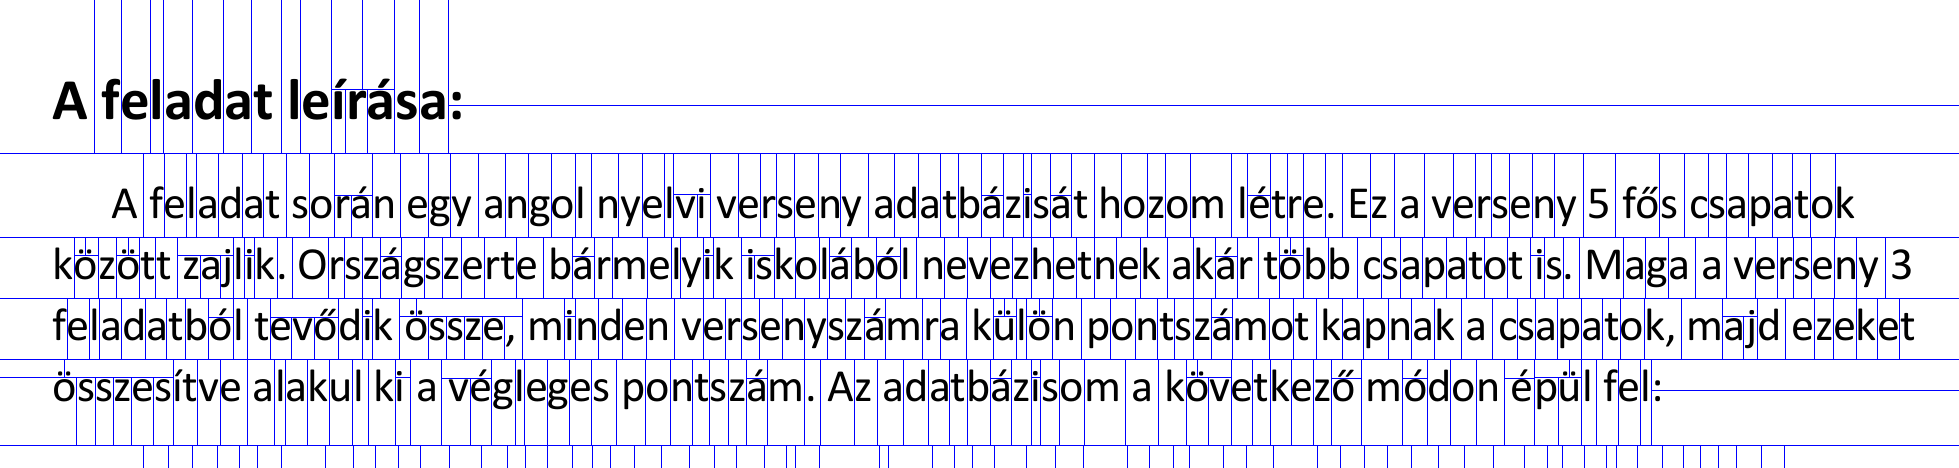
\includegraphics[width=\textwidth]{images/splitted.png}
\caption{A felosztással kapott eredmények egy részlete}
\label{fig:splitted}
\end{figure}

\Section{Összefüggő képterületek detektálása}

A karakterek elkülönítése szempontjából problémát jelent a kerning. Ez arra szolgál, hogy az egymáshoz szebben, arányosabban illeszthető karaktereknél korrigálja az egyenközű egymás után illesztést. Egy szélsőséges eseteként az \emph{fl} és \emph{ff} betűkből képzett ligatúrák szerepelnek.

A feldolgozás és karakterfelismerés szempontjából ezek külön figyelmet igényelnek.
A probléma egy lehetséges megoldását az adja, hogy ha az egyenesekkel történő felosztás helyett olyan algoritmust használunk, amely inkább az összefüggő képterületeket keresi meg, vagyis gyakorlatilag klaszterezi a képet. (A klaszterek ebben az értelmezésben többségében a karaktereket, vagy az azokhoz hasonlóan összefüggő képterületeket jelenti.)

Az összefüggő képpontok csoportjának (\textit{blob}-oknak) a keresése feltételez valamilyen hasonlóságot a képpontokra nézve. Ez esetben ez két összetevőből adódik. Egyrészt küszöbölés segítségével meg kell állapítani, hogy a képpont világos vagy sötét-e. Mivel PDF-ből konvertált képről van szó, ezért a kép kontrasztos, és többségében csak az élsimításból adódó zajokat tartalmazza, így ez egyszerűen, akár 128-as küszöbértékkel végezhető egy tipikus dokumentum esetén.

A másik összetevő a szomszédsági viszony megadása. Feltételezzük, hogy az algoritmus csak a sor- és oszlop szerinti szomszédságot veszi figyelembe. Így egy egyszerű szélességi bejárással meghatározhatók az összefüggő csoportok.
Maga az algoritmus tulajdonképpen egy színkitöltő algoritmus (\textit{floodfill}) egyszerűsített változata lesz így \cite{floodfill}.
A \texttt{blob\_shapes.ipynb} nevű munkafüzetben \texttt{find\_blob} néven került implementálásra.
Ez paraméterként az alábbi objektumokat várja.
\begin{itemize}
\item \texttt{image}: A feldolgozandó kép \texttt{NumPy} tömb formájában.
\item \texttt{start\_point}: A szélességi bejárás kezdőpontja (sor, oszlop) indexpár formájában.
\item \texttt{threshold}: A küszöböléshez használt érték.
\item \texttt{is\_visited}: Egy \textit{NumPy} tömb, amely logikai értékeket tartalmaz, és azt tárolja, hogy mely képpontok kerültek már vizsgálatra.
\end{itemize}
Mivel Python-ban az objektumok referencia szerint adódnak át, így az \texttt{is\_visited} paraméter egyúttal kimeneti értékként is kezelendő.
Maga a függvény elsődleges visszatérési értéke a \textit{blob}-hoz tartozó képpontoknak a koordinátái lesznek.

Az algoritmus, amelyik a képen lévő összes összefüggő foltot megkeresi az alábbi formában néz ki.
\begin{python}
def find_blobs(image):
    """
    Find the blobs on the image.
    :param image: a two dimensional NumPy array
    :return: list of the collected blobs
    """
    blobs = []
    threshold = 128
    is_visited = np.zeros(image.shape, dtype=int)
    n_rows, n_columns = image.shape
    for i in range(n_rows):
        for j in range(n_columns):
            if is_visited[i, j] == False and image[i, j] < threshold:
                blob = find_blob(image, (i, j), threshold, is_visited)
                blobs.append(blob)
            is_visited[i, j] = True
    return blobs
\end{python}

A kapott eredmények ellenőrzéséhez a munkafüzetben kirajzolásra kerültek a foltok befoglaló téglatestjei. Ezt  egy mintakép részletére \aref{fig:bounded_boxes}. ábrán láthatjuk.

\begin{figure}[h!]
\centering
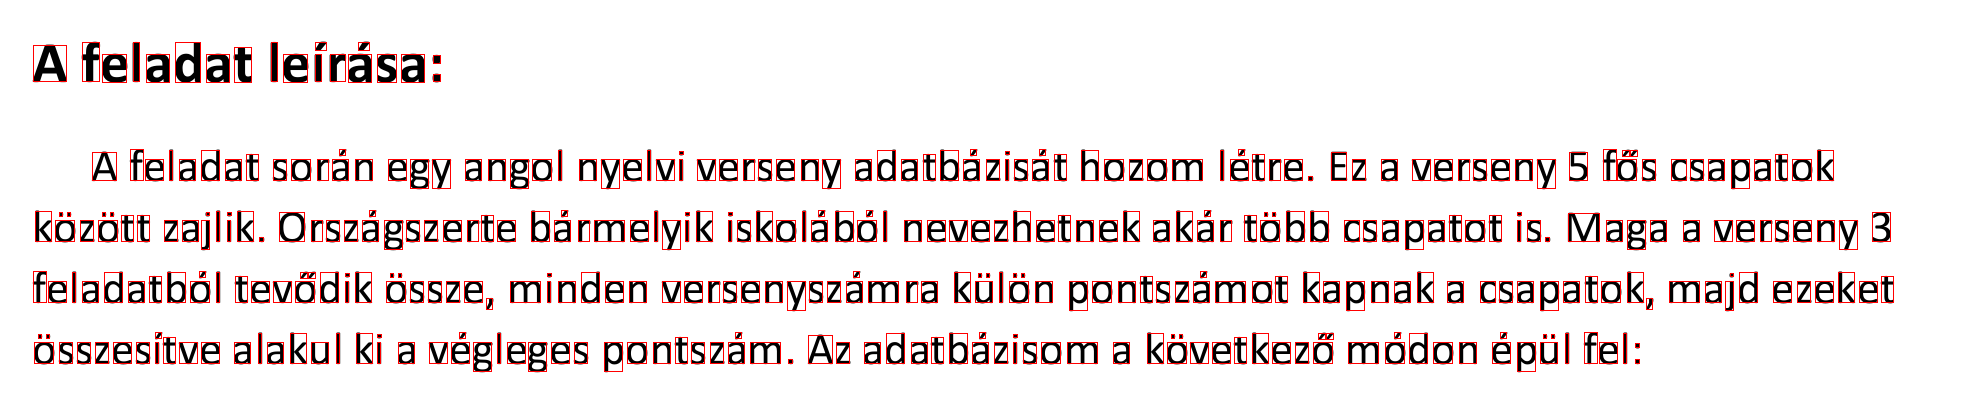
\includegraphics[width=\textwidth]{images/bounded_boxes.png}
\caption{Az összefüggő foltokhoz tartozó befoglaló téglatestek}
\label{fig:bounded_boxes}
\end{figure}

A foltok pontjainak ismeretében már további elemzési lehetőségek is adódtak. A munkafüzetben elemzésre került foltokhoz tartozó képpontok számának, a befoglaló téglatestjeik szélességének és magasságának az eloszlásai.

Feltételezhető, hogy a foltok ismeretében nagyobb megbízhatósággal elvégezhető a karakterek felismerése.
Ehhez a \texttt{render\_blob} függvény a foltot egy adott méretű képterületre kirajzolja.
\begin{python}
def render_blob(blob, image_size):
    """
    Render the blob to a fixed size image.
    :param blob: list of pixel coordinates
    :param image_size: size of the rendered image
    :return: a NumPy array with 0 and 1 values
    """
    image = np.zeros(image_size, dtype=int)
    min_row = min([i for i, _ in blob])
    min_column = min([j for _, j in blob])
    for row, column in blob:
        image[row - min_row, column - min_column] = 1
    return image
\end{python}
A rögzített méret miatt a karakterek, mint képek, a környező zajok nélkül összehasonlíthatóak.
Az összehasonlításokhoz a vizsgálatokban egy egyszerű mátrixtávolság-számítás került megvalósításra az alábbi formában.
\begin{python}
def compare_blob(blob_1, blob_2):
    """
    Calculate the distance of the blobs.
    :param blob_1: list of blob pixels
    :param blob_2: list of blob pixels
    :return: distance of the blobs
    """
    image_1 = render_blob(blob_1, (50, 50))
    image_2 = render_blob(blob_2, (50, 50))
    distance = np.sum(np.sum(np.abs(image_1 - image_2)))
    return distance
\end{python}
Az $50\times50$-es képméretet az eloszlások alapján egyszerűen lehetett becsülni.

Ezzel a metrikával már osztályozni lehet a foltokat egy referencia folthoz viszonyított távolság alapján.
Legyen ez a folt, most egy \emph{a} karakterhez tartozó folt.
\Aref{fig:a_distances}. ábrán az összes foltnak a referencia folttól való távolságainak a hisztogramja látható (20 intervallumra osztva a tartományt).

\begin{figure}[h!]
\centering
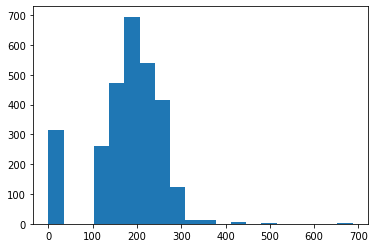
\includegraphics[width=\textwidth]{images/a_distances.png}
\caption{Az \emph{a} karakterhez tartozó referencia folttól való távolságok hisztogramja}
\label{fig:a_distances}
\end{figure}

Az értékekből az olvasható le, hogy a $[0, 100]$ intervallumot a távolságokra nézve gyakorlatilag bárhol ketté lehet vágni a közepe felé.
Ezt válasszuk meg például 60-nak.
Ekkor az ezekhez tartozó foltokat sárga színnel kijelölve \aref{fig:a_characters}. ábrán láthatjuk.

\begin{figure}[h!]
\centering
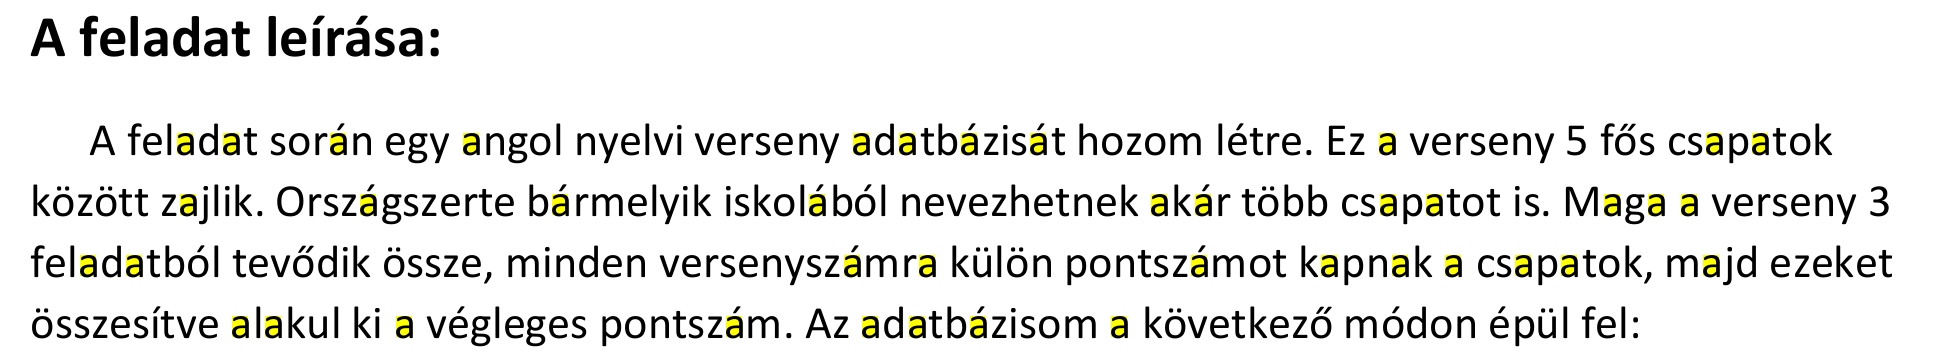
\includegraphics[width=\textwidth]{images/a_characters.png}
\caption{A mintában sárgával kijelölt \emph{a} karakterek}
\label{fig:a_characters}
\end{figure}

Érdemes azt észrevenni, hogy a \textbf{feladat} szóban szereplő \textbf{a} karakter nem lett kijelölve.
Ez a miatt van, mert a küszöbérték aránylag alacsony értékre lett beállítva, illetve mert a távolságszámítás önmagában csak a közeli egyezés, a kisebb eltérések figyelmen kívül hagyására alkalmas.

A módszer kimondottan előnyös több szempontból is.
Egyrészt, nem feltételezi, hogy a karakterek egyáltalán sorokba lennének rendezve.
Másrészt, a karakterek között lehet olyan értelemben átfedés, amely semmilyen felosztásra épülő befoglaló téglatestes módszerrel nem lenne kezelhető.
